\section{Process Management}

\noindent
Our SOS implementation supports up to 512 processes.
These processes are managed by a static array.
We synchronize access to this static array by using a process
management server (PM server). When SOS threads desire to manipulate the state of SOS
processes, they perform an IPC call to the process management server's 
endpoint.
\\

\subsection{Process ID Allocation}

\noindent
Process ids are simply the index of a given process in the process management static
array. Note that the process management thread and the file server thread 
don't have entries in this array, so syscalls invokes by users cannot wait or kill
these system processes.
\\

\subsection{Process Creation}

\noindent
The thread\_create syscall calls into the PM server in order to create a new
thread. When creating a new thread, the PM server first allocates resources for
and starts up a new SOS thread. This is done similarly to the starter code, 
with some additions to cleanup failed attempts at starting a new thread. 
The newly created thread then begins executing and allocates resources
for a user thread which executes the desired app. When thread\_create is called,
the resources for an old SOS thread may be reused as described below. Newly created
SOS threads get added to the first free entry in the process management array and
uses its index in the array as its process ID.
\\

\subsection{Blocking and Waiting for Access to Devices}

\noindent
Sleeping and waiting for device access is also handled by the PM
server. For example, a process desiring to sleep will
make an IPC call to the PM server, specifying how long it
wishes to sleep for.
\\

\noindent
Within the process management loop, a process desiring
to sleep will be suspended and a timeout will be registered that will call
back into PM server at the appropriate time to wake the thread
back up.
\\

\noindent
A thread requesting access to a device will pass the id of the device which
it wants to access (currently there is only a console device however).
If the device is already in use, the process is put into a queue and suspended.
\\

\noindent
Queues to access devices and sleeping is handled inside the PM
server so that killing a process can be easily implemented, as discussed in
the next section.
\\

\subsection{Killing a Process}

\begin{figure}[h]
    \centering
    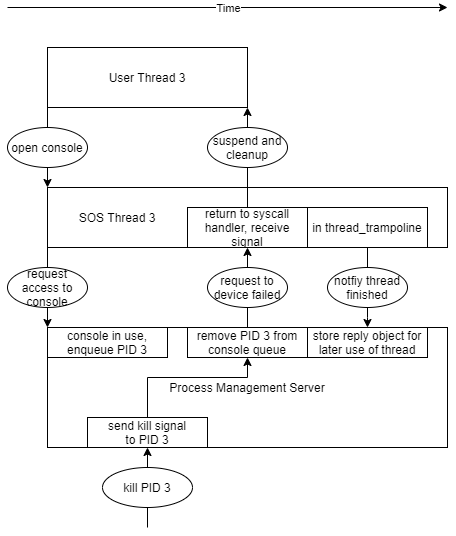
\includegraphics[width=100mm]{process_management_example.png}
    \caption{Process kill example}
    \label{fig:process_management}
\end{figure}

\noindent
Each SOS 'syscall handler' thread, that is, the threads paired with user-level
processes, have a notification object bound to their TCB. The PM
server is given a minted capability to this notification object which it used
to signal to a thread that it is being killed. The advantage of this design is
that it is relatively easy for the SOS syscall handler thread to cleanup
appropriate user level thread resources itself before calling into
the PM server to have itself cleaned up. The only problem
with this approach is that SOS threads which are blocked for an arbitrary amount
of time (sleeping, waiting for access to a device) will not immediately respond to
the kill signal, as the signal will only be received when seL4\_Recv is called
in the SOS thread's syscall handler loop. This blocking for device access and 
sleeping are both handled inside the process management loop. After signalling
the process being killed, the PM server will check to see whether the process
being killed is sleeping or waiting for a device. If it is, then the process
will be prematurely woken up and will respond to the kill signal when it 
again calls seL4\_Recv after responding to the syscall that it was processing.
The running time of other syscalls (even ones that block, such as IO calls) are 
assumed to be sufficiently short so that no special action needs to be taken. The
process will complete whatever system call it is performing, call seL4\_Recv,
and receive the signal that it is being killed.
\\

\noindent
When a kill occurs, a user process's syscall handling SOS thread cleans up
all the resources associated with the user thread, but the PM server doesn't
actually clean the resources associated with the SOS thread. We've modified 
the thread\_trampoline code in threads.c so that when a SOS thread returns to the
trampoline, it calls back into the PM server. When this happens, the PM server 
marks the thread as free and stores the reply object to the thread. When a 
user calls thread\_create, this old SOS thread will be reused if it exited 
sufficiently long ago (currently 5 seconds) to avoid causing race conditions.
To reuse the thread, the PM server simply responds to the saved reply object the
address of the buffer containing the name of the app to be started. If this thread
is killed it will again return to thread\_trampoline and call into the PM server,
indicating it is ready for reuse.
\\

\noindent
The primary advantage of this approach is that an explicit bitfield keeping track
of free virtual addresses for new SOS stacks and IPC buffers doesn't need to be 
maintained, and SOS doesn't have to keep reclaiming and allocating the same
resources. It is true that if session of SOS usage uses $x$ number of threads then
resources for all those $x$ threads will remain allocated until the system is
rebooted, but it is also true that if $x$ threads were used in the past, that many
could be used again.
\\
